\documentclass{article}
\usepackage{amsmath}
\usepackage{amssymb}
\usepackage{tikz}
\usetikzlibrary[patterns]
\usetikzlibrary{shapes.geometric}
\usepackage{pgfplots}
\pgfplotsset{compat=1.18}
\usepackage{xcolor,colortbl}

\begin{document}

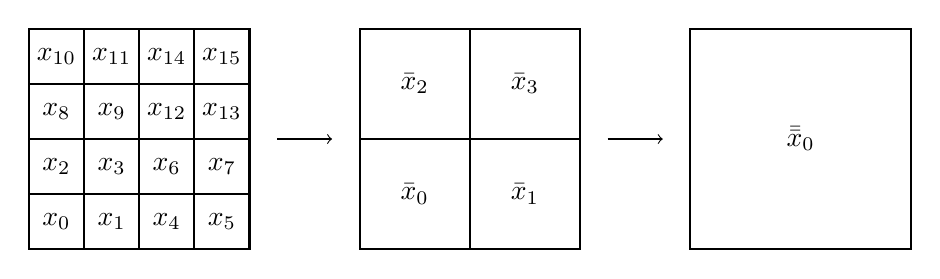
\begin{tikzpicture}[scale=0.7]

    % The grid
	\draw[step=1.0,black,thick] (0,0) grid (4,4);
	\draw[black, thick] (0,0) -- (4,0) -- (4,4) -- (0,4) -- cycle;

	% The Space Filling Curve indices
	\draw (0.5,0.5) node{$x_{0}$};
	\draw (1.5,0.5) node{$x_{1}$};
	\draw (0.5,1.5) node{$x_{2}$};
	\draw (1.5,1.5) node{$x_{3}$};
	\draw (2.5,0.5) node{$x_{4}$};
	\draw (3.5,0.5) node{$x_{5}$};
	\draw (2.5,1.5) node{$x_{6}$};
	\draw (3.5,1.5) node{$x_{7}$};
	\draw (0.5,2.5) node{$x_{8}$};
	\draw (1.5,2.5) node{$x_{9}$};
	\draw (0.5,3.5) node{$x_{10}$};
	\draw (1.5,3.5) node{$x_{11}$};
	\draw (2.5,2.5) node{$x_{12}$};
	\draw (3.5,2.5) node{$x_{13}$};
	\draw (2.5,3.5) node{$x_{14}$};
	\draw (3.5,3.5) node{$x_{15}$};

	%Arrow
	\draw[black, ->] (4.5,2) -- (5.5,2);

	% The grid of the first coarsening
	\draw[step=2.0,black,thick] (6,0) grid (10,4);
	\draw[black, thick] (6,0) -- (10,0) -- (10,4) -- (6,4) -- cycle;

	\draw (7,1) node{$\Bar{x}_{0}$};
	\draw (9,1) node{$\Bar{x}_{1}$};
	\draw (7,3) node{$\Bar{x}_{2}$};
	\draw (9,3) node{$\Bar{x}_{3}$};

	%Arrow
	\draw[black, ->] (10.5,2) -- (11.5,2);

	% The grid of the second coarsening
	\draw[black, thick] (12,0) -- (16,0) -- (16,4) -- (12,4) -- cycle;

	\draw (14,2) node{$\Bar{\Bar{x}}_{0}$};

\end{tikzpicture}

\end{document}